%%%%%%
%%%%%%%%%%%%%%%%%%%%%%%%%%%%%% Title Page Info %%%%%%%%%%%%%%%%%%%%%%%%%%%%%%%%%%%%%%%%%%%
%%%%%%%%%%%%%%%%%%%%%%%%%%%%%%%%%%%%%%%%%%%%%%%%%%%%%%%%%%%%%%%%%%%%%%%%%%%%%%%%%%%%%%%%%%

\documentclass[aspectratio=169,compress]{beamer}
\mode<presentation> 

%\usetheme{Warsaw}
\usetheme{Antibes}
%\usecolortheme{beaver}
\usecolortheme[rgb={0.7,0.0,0.0}]{structure}
%\useoutertheme[subsection=false]{miniframes}

\makeatletter
\setbeamertemplate{headline}
{%
    \begin{beamercolorbox}[wd=\paperwidth,colsep=1.5pt]{upper separation line head}
    \end{beamercolorbox}
    \begin{beamercolorbox}[wd=\paperwidth,ht=2.5ex,dp=1.125ex,%
      leftskip=.3cm,rightskip=.3cm plus1fil]{title in head/foot}
      \usebeamerfont{title in head/foot}\insertshorttitle
    \end{beamercolorbox}
    \begin{beamercolorbox}[wd=\paperwidth,ht=2.5ex,dp=1.125ex,%
      leftskip=.3cm,rightskip=.3cm plus1fil]{section in head/foot}
      \usebeamerfont{section in head/foot}%
      \ifbeamer@tree@showhooks
        \setbox\beamer@tempbox=\hbox{\insertsectionhead}%
        \ifdim\wd\beamer@tempbox>1pt%
          \hskip2pt\raise1.9pt\hbox{\vrule width0.4pt height1.875ex\vrule width 5pt height0.4pt}%
          \hskip1pt%
        \fi%
      \else%  
        \hskip6pt%
      \fi%
      \insertsectionhead
    \end{beamercolorbox}
% Code for subsections removed here
}
\makeatother


% define
% PAra las diapositivas concentradoras de muchos proyectos, no es conveniente la plantilla de puntitos, se debe utilizar otra
%\usepackage{beamerouterthememiniframes} % Para los puntitos 
\setbeamertemplate{footline}[frame number]{}

% include packages
\usepackage{minted}
\usepackage{subfigure}
\usepackage{multicol}
\usepackage{amsmath}
\usepackage{epsfig}
\usepackage{graphicx}
\usepackage[all,knot]{xy}
\usepackage{algorithmic}
\xyoption{arc}
\usepackage{url}
\usepackage{multimedia}
\usepackage{hyperref}
\usepackage{tikz}

\usepackage{pgfpages}
\setbeameroption{hide notes} % Only slides
%\setbeameroption{show only notes} % Only notes
%\setbeameroption{show notes on second screen=right} % Both

\title{Proyectos Dirigidos}
%\title{Proyectos selectos de visión por computadora y aprendizaje automático del Laboratorio de Sistemas Inteligentes de la UPV} % TecMTY
%\title{Recopilación de 10 años de investigación del Laboratorio de Sistemas Inteligentes de la UPV}

\author{Dr. Marco Aurelio Nu\~no Maganda}
\institute{Universidad Politécnica de Victoria\\ Laboratorio de Sistemas Inteligentes \\
mnunom@upv.edu.mx  \vspace{.25cm} }

\date{Octubre 2022}
%\textbf{nmaganda@ccc.inaoep.mx}

%%%%%%%%%%%%%%%%%%%%%%%%%%%%%%%%%%%%%%%%%%%%%%%%%%%%%%%%%%%%%%%%%%%%%%%%%%%%%%%%%%%%%%%%%%
%%%%%%%%%%%%%%%%%%%%%%%%%%%%%% Begin Your Document %%%%%%%%%%%%%%%%%%%%%%%%%%%%%%%%%%%%%%%
%%%%%%%%%%%%%%%%%%%%%%%%%%%%%%%%%%%%%%%%%%%%%%%%%%%%%%%%%%%%%%%%%%%%%%%%%%%%%%%%%%%%%%%%%%

 

%\usepackage[backend=biber,maxcitenames=50,maxbibnames=50,sorting=ydmdddnt]{biblatex}
\usepackage[backend=biber,maxcitenames=50,maxbibnames=50,sorting=none]{biblatex}






%\renewrobustcmd{\mkbibfootnote}{\normalsize\footnotemark\footnotetext}
\setbeamerfont{footnote}{size=\tiny}






\newcommand{\ArchivoPrincipal}{Todos}
\newcommand{\ArchivoSecundario}{Bibliografia}


%Append keywords to identify different bibliography entries.
\DeclareSourcemap{
  \maps[datatype=bibtex, overwrite]{
    \map{
      \perdatasource{\ArchivoPrincipal.bib}
      \step[fieldset=KEYWORDS, fieldvalue=primary, append]
    }
    \map{
      \perdatasource{\ArchivoSecundario.bib}
      \step[fieldset=KEYWORDS, fieldvalue=secundary, append]
    }    
  }
}


\addbibresource{\ArchivoPrincipal.bib}
\addbibresource{\ArchivoSecundario.bib}

\usepackage{listings}
 
 \AtBeginSection[]
{
    \begin{frame}
        \frametitle{Outline}
        \tableofcontents[currentsection]
    \end{frame}
}

\makeatletter
\def\@makefnmark{}
\makeatletter
\setbeamertemplate{footnote}{%
  \parindent 1em\noindent
  \raggedright
  *  
  \insertfootnotetext\par
}


\newcommand{\EntradaBibtex}{InvalidEntry}

\begin{document}










\section{2024_GerminadorAutomatico}

\renewcommand{\EntradaBibtex}{GerminadorAutomatico_EstadiasMecatronica_UPV_2024}

\begin{frame}{\citetitle{\EntradaBibtex}$^*$ (1)}
\begin{block}{Motivación} 
 Un germinador favorece el desarrollo de semillas en condiciones adecuadas (temperatura y humedad). Su automatización es importante para incentivar el cultivo de alimentos en casa
\end{block} 

\begin{itemize}
\item Se agregan sensores, actuadores y software para monitorear el desarrollo de los brotes de manera remota
\item Una cámara captura fotos de los brotes en intervalos de tiempo regulares
\item Los sensores de humedad y temperatura permiten obtener retroalimentación de las condiciones del entorno de los brotes
\item Un sistema de bombeo de agua permite mantener la humedad en niveles óptimos 
\end{itemize}

\footfullcite*{\EntradaBibtex}
\end{frame}

\begin{frame}{\citetitle{\EntradaBibtex} (2)}

\begin{columns}

% Column 1
\column{.6\linewidth}

\begin{center}
	\begin{tabular}{cc}
		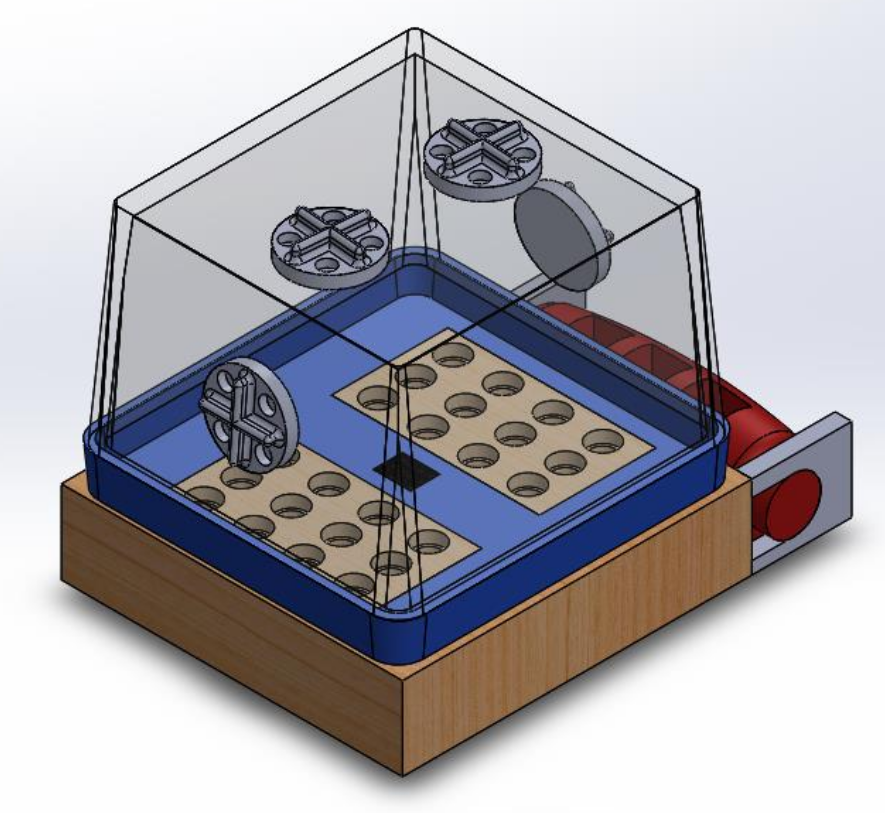
\includegraphics[width=0.5\linewidth]{2024_GerminadorAutomatico/figs/PrototipoGerminador.png}&
		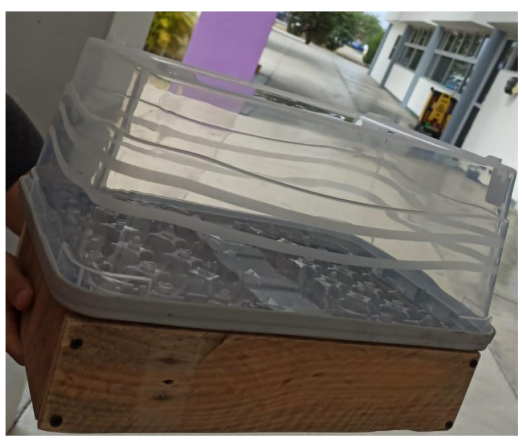
\includegraphics[width=0.5\linewidth]{2024_GerminadorAutomatico/figs/GerminadorFinal.png} \\
	\end{tabular}
\end{center}
\column{.4\linewidth}
	\begin{tabular}{c}
		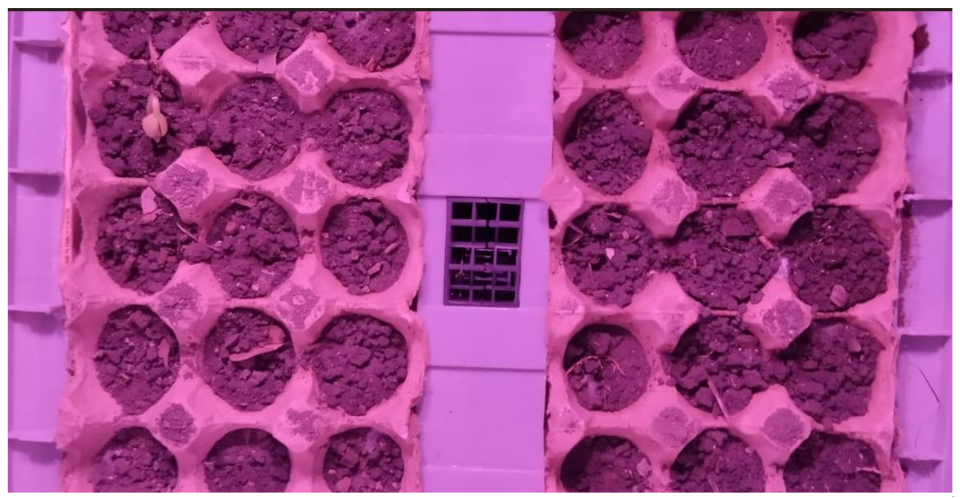
\includegraphics[width=0.9\linewidth]{2024_GerminadorAutomatico/figs/SemillasenGerminador.png} \\
		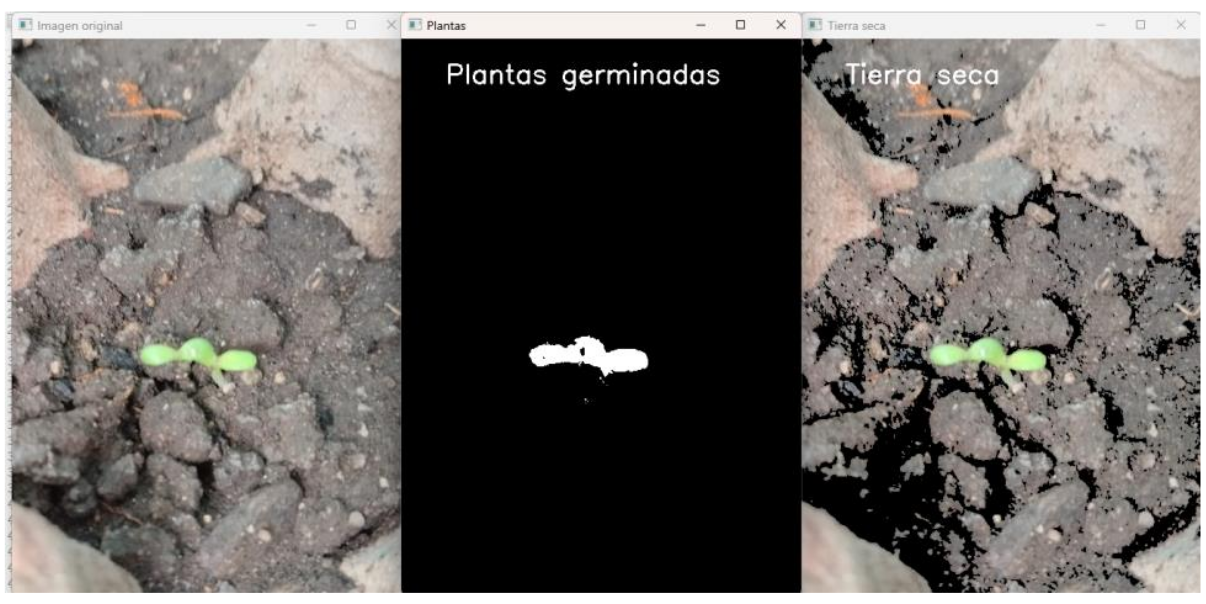
\includegraphics[width=0.9\linewidth]{2024_GerminadorAutomatico/figs/ModuloVision.png} \\
	\end{tabular}

\end{columns}

\end{frame}

\begin{frame}{\citetitle{\EntradaBibtex} (3)}
\begin{itemize}
	\item Se seleccionaron plantas de rápido crecimiento, con la finalidad de obtener resultados significativos. Específicamente, los cultivos seleccionados fueron frijol, lenteja, cilandro y lechuga.
    %\item El germinador automático permite garantizar un crecimiento saludable de las plantas al monitorear los brotes de manera continua. 
    \item El monitoreo visual remoto facilita la detección temprana de problemas y la toma de decisiones informadas.
    \item El sistema propuesto permitirá la evaluación de las mismas condiciones de temperatura/humedad/iluminación con diferentes variedades de semillas, o variar las condiciones con sobre la misma variedad de semilla.  
    \item Con respecto al módulo de visión, se desea determinar de manera precisa el número de hojas del brote, con la finalidad de indicar al usuario del momento adecuado para hacer el trasplante o se requiera atención especial.
\end{itemize}
\end{frame}





\end{document}
